\section{Аналитический метод криптоанализа.}

\task{Найти минимальную сложность нахождения ключа в схеме

\begin{tikzpicture}[>=latex]
{\centering
\draw[thick, ->] (0,0) node[left] {от} -- (1,0);
\draw (1,-0.5) rectangle node[midway] {$A$} (3.5,0.5);
\draw[thick, ->] (3.5,0) -- (4.5,0) node[right] {шт};
}
\end{tikzpicture}

Ключом является невырожденная двоичная матрица $А$ размером~$n~\cdot~n$. Сравнить со сложностью МПП.}

При решении СЛАУ методом Гаусса сложность оценивается в $\frac{n^3}{3}$~операций. Количество операций, необходимое для проверки одного ключа, равно $p = (n + (n - 1)) \cdot n = 2 n ^ 2 - n$ -- такое количество операций сложения и умножения нужно проделать для умножения вектора на квадратную матрицу. Было установлено, что:
$$|K| = \prod_{i = 0} ^ {n - 1} 2^n - 2^i = (2 ^ n) ^ {n} + ... = O(2 ^ {n^2})$$
Следовательно, сложность МПП:
$$E\tau = p \frac{|K| + 1}{2} = (2 n ^ 2 - n) \frac{2 ^ {n^2} + ...}{2} = O (n^2 \cdot 2 ^ {n^2})$$

Пусть $n = 10$, тогда для МПП потребуется порядка $10^2 \cdot 2 ^ {10^2} \approx 10^{32.10}$ операций, тогда как для аналитического метода получится $\frac{10^3}{3} \approx 3 \cdot 10^2$ операций.

\task{Для ЛРП, задаваемой с помощью характеристического многочлена \\ \\
$F(x) = x^4 \oplus x^2 \oplus x \oplus 1$, построить ЛРС, определить матрицу $A$, и для выходной (после 4-х тактов работы ЛРС) последовательности $\gamma = (1, 0, 1, 0) $ найти начальное заполнение регистра.}

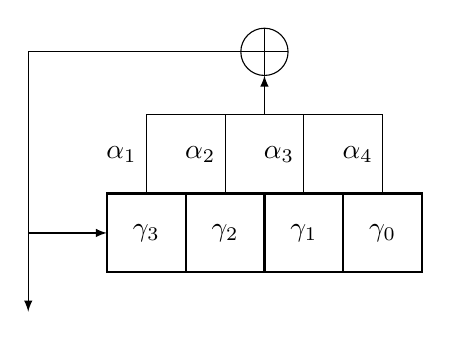
\begin{tikzpicture}[>=latex]
{\centering
\draw[thick] (1,-0.5) rectangle node[midway] {$\gamma_3$} (2,0.5);
\draw[thick] (2,-0.5) rectangle node[midway] {$\gamma_2$} (3,0.5);
\draw[thick] (3,-0.5) rectangle node[midway] {$\gamma_1$} (4,0.5);
\draw[thick] (4,-0.5) rectangle node[midway] {$\gamma_0$} (5,0.5);

\draw[-] (1.5, 0.5) -- node[left] {$\alpha_1$} (1.5, 1.5);
\draw[-] (2.5, 0.5) -- node[left] {$\alpha_2$} (2.5, 1.5);
\draw[-] (3.5, 0.5) -- node[left] {$\alpha_3$} (3.5, 1.5);
\draw[-] (4.5, 0.5) -- node[left] {$\alpha_4$} (4.5, 1.5);
\draw[-] (1.5, 1.5) -- (4.5, 1.5);
\draw[->] (3, 1.5) -- (3, 2);
% xor
\draw (3, 2.3) circle (0.3);
\draw[-] (2.7, 2.3) -- (3.3, 2.3);
\draw[-] (3, 2.6) -- (3, 2);
%
\draw[-] (2.7, 2.3) -- (0, 2.3);
\draw[->] (0, 2.3) -- (0, -1);
\draw[->] (0, 0) -- (1, 0);
}
\end{tikzpicture}

Из характеристической функции следует, что $\alpha_1 = 1, \alpha_2 = 1, \alpha_3 =~0, \alpha_4 =~1$. Тогда $\gamma_4 = 1 \cdot \gamma_0 + 0 \cdot \gamma_1 + 1 \cdot \gamma_2 + 1 \cdot \gamma_3$. Значит, матрица $A$ = 
$
\begin{bmatrix}
0 &1 &0 &0\\
0 &0 &1 &0 \\
0 &0 &0 &1 \\
1 &0 &1 &1
\end{bmatrix}
$. Решим следующее уравнение: $A^4 \gamma ^T (0) = \gamma ^ T.$

$A^4$ = 
$
\begin{bmatrix}
0 &0 &1 &0\\
0 &0 &0 &1 \\
1 &0 &1 &1 \\
1 &1 &1 &2
\end{bmatrix} ^ 2
$ =
$
\begin{bmatrix}
1 &0 &1 &1\\
1 &1 &1 &2 \\
2 &1 &3 &3 \\
3 &2 &4 &6
\end{bmatrix}
$ =
$
\begin{bmatrix}
1 &0 &1 &1\\
1 &1 &1 &0 \\
0 &1 &1 &1 \\
1 &0 &0 &0
\end{bmatrix}
$

$
\left[
  \begin{matrix}
1 &0 &1 &1\\
1 &1 &1 &0 \\
0 &1 &1 &1 \\
1 &0 &0 &0
  \end{matrix}
  \left|
    \,
    \begin{matrix}
      1  \\
      0  \\
      1  \\
      0  \\
    \end{matrix}
  \right.
\right]
$
$\sim$
$
\left[
  \begin{matrix}
0 &0 &1 &0\\
0 &1 &0 &0 \\
0 &0 &0 &1 \\
1 &0 &0 &0
  \end{matrix}
  \left|
    \,
    \begin{matrix}
      0  \\
      0  \\
      1  \\
      0  \\
    \end{matrix}
  \right.
\right]
$
$\sim$
$
\left[
  \begin{matrix}
	1 &0 &0 &0 \\
	0 &1 &0 &0 \\
	0 &0 &1 &0 \\
	0 &0 &0 &1
  \end{matrix}
  \left|
    \,
    \begin{matrix}
      0  \\
      0  \\
      0  \\
      1  \\
    \end{matrix}
  \right.
\right]
$

Следовательно, $\gamma(0) = (0, 0, 0, 1)$.

\task{Объяснить равенства (4.11) и (4.12).}

Пусть $f$ имеет следующую структуру: $$f(\gamma_n, \gamma_{n+1}, ..., \gamma_{n + r - 1}) = \gamma_n \oplus g(\gamma_{n+1}, \gamma_{n+1}, ..., \gamma_{n + r - 1}).$$

\noindent Тогда: $$f(0, x_2, ...,x_r) \oplus f(1, x_2, ...,x_r) = 0 \oplus g(x_2, ...,x_r) \oplus 1 \oplus g(x_2, ...,x_r) = 1$$

\noindent Следовательно, $f(0, x_2, ...,x_r) = 1 \oplus f(1, x_2, ...,x_r).$


Равенство $f(x_1, x_2, ...,x_r) = x_1 f(1, x_2, ...,x_r) \oplus (1 \oplus x_1) f(0, x_2, ...,x_r)$ проверяется непосредственной подстановкой $x_1$.
В самом деле, при $x_1 =~0$ первое слагаемое обращается в ноль, и имеем $f(0, x_2, ...,x_r) = f(0, x_2, ...,x_r)$. А при $x_1 = 1$ -- второе: $f(1, x_2, ...,x_r) = f(1, x_2, ...,x_r)$

\task{Построить графы отображений для РС, обратные связи которых задаются функциями от 4 переменных: \\
\(f_1 = x_2 \oplus x_3 \), \(f_2 = x_1 \oplus x_2 \oplus x_3\), \( f_3 = x_3 \oplus x_2*x_4\), \(f_4 = x_1 \oplus x_3*x_4\), \(f_5 = x_1*x_3 \oplus x_2*x_4\).\\
Прокомментировать результаты. }

ЛРС $F_1 : (x_1, x_2, x_3, x_4) \rightarrow (x_2, x_3, x_4, x_2 \oplus x_3)$

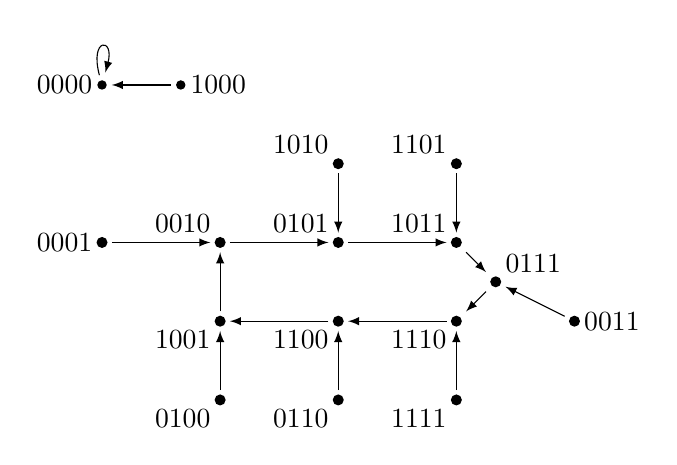
\begin{tikzpicture}[>=latex]
{\centering
\node (0000) at (0, 0) {};
\fill (0000)[right] circle (0.06) node[left] {$0000$};
\path[->] (0000) edge [loop above] node {} ();

\node (1000) at (1, 0) {};
\fill (1000)[left] circle (0.06) node[right] {$1000$};
\path[->] (1000) edge node {} (0000);

\node (0001) at (0, -2) {};
\fill (0001)[right] circle (0.07) node[left] {$0001$};
\node (0010) at (1.5, -2) {};
\fill (0010)[left] circle (0.07) node[above left] {$0010$};
\node (0101) at (3, -2) {};
\fill (0101)[left] circle (0.07) node[above left] {$0101$};
\node (1011) at (4.5, -2) {};
\fill (1011)[left] circle (0.07) node[above left] {$1011$};
\node (0111) at (5, -2.5) {};
\fill (0111)[left] circle (0.07) node[above right] {$0111$};

\node (1110) at (4.5, -3) {};
\fill (1110)[left] circle (0.07) node[below left] {$1110$};
\node (1100) at (3, -3) {};
\fill (1100)[left] circle (0.07) node[below left] {$1100$};
\node (1001) at (1.5, -3) {};
\fill (1001)[left] circle (0.07) node[below left] {$1001$};

\node (0100) at (1.5, -4) {};
\fill (0100)[left] circle (0.07) node[below left] {$0100$};
\node (0110) at (3, -4) {};
\fill (0110)[left] circle (0.07) node[below left] {$0110$};
\node (1111) at (4.5, -4) {};
\fill (1111)[left] circle (0.07) node[below left] {$1111$};
\node (0011) at (6, -3) {};
\fill (0011)[left] circle (0.07) node[right] {$0011$};

\node (1010) at (3, -1) {};
\fill (1010)[left] circle (0.07) node[above left] {$1010$};
\node (1101) at (4.5, -1) {};
\fill (1101)[left] circle (0.07) node[above left] {$1101$};

\path[->] (0001) edge node {} (0010);
\path[->] (0010) edge node {} (0101);
\path[->] (0101) edge node {} (1011);
\path[->] (1011) edge node {} (0111);
\path[->] (0111) edge node {} (1110);
\path[->] (1110) edge node {} (1100);
\path[->] (1100) edge node {} (1001);
\path[->] (1001) edge node {} (0010);
\path[->] (1010) edge node {} (0101);
\path[->] (1101) edge node {} (1011);
\path[->] (0011) edge node {} (0111);
\path[->] (1111) edge node {} (1110);
\path[->] (0110) edge node {} (1100);
\path[->] (0100) edge node {} (1001);

}
\end{tikzpicture}

\noindent Данный граф имеет структуру "циклы с подходами". Длины циклов: 1, 7. Это отображение не является взаимно однозначным.

\medskip

ЛРС $F_2 : (x_1, x_2, x_3, x_4) \rightarrow (x_2, x_3, x_4, x_1 \oplus x_2 \oplus x_3)$

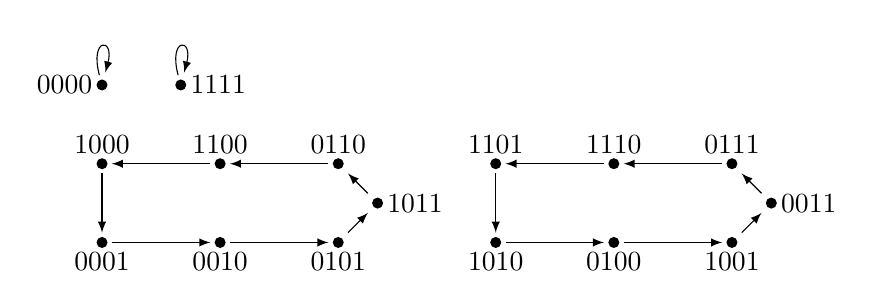
\begin{tikzpicture}[>=latex]
{\centering
\node (0000) at (0, 0) {};
\fill (0000)[right] circle (0.07) node[left] {$0000$};
\path[->] (0000) edge [loop above] node {} ();

\node (1111) at (1, 0) {};
\fill (1111)[left] circle (0.07) node[right] {$1111$};
\path[->] (1111) edge [loop above] node {} ();

\node (1000) at (0, -1) {};
\fill (1000)[left] circle (0.07) node[above] {$1000$};
\node (1100) at (1.5, -1) {};
\fill (1100)[left] circle (0.07) node[above] {$1100$};
\node (0110) at (3, -1) {};
\fill (0110)[left] circle (0.07) node[above] {$0110$};
\node (1011) at (3.5, -1.5) {};
\fill (1011)[left] circle (0.07) node[right] {$1011$};


\node (0111) at (8, -1) {};
\fill (0111)[left] circle (0.07) node[above] {$0111$};
\node (1110) at (6.5, -1) {};
\fill (1110)[left] circle (0.07) node[above] {$1110$};
\node (1101) at (5, -1) {};
\fill (1101)[left] circle (0.07) node[above] {$1101$};
\node (1010) at (5, -2) {};
\fill (1010)[left] circle (0.07) node[below] {$1010$};
\node (0100) at (6.5, -2) {};
\fill (0100)[left] circle (0.07) node[below] {$0100$};
\node (1001) at (8, -2) {};
\fill (1001)[left] circle (0.07) node[below] {$1001$};
\node (0011) at (8.5, -1.5) {};
\fill (0011)[left] circle (0.07) node[right] {$0011$};

\node (0001) at (0, -2) {};
\fill (0001)[right] circle (0.07) node[below] {$0001$};
\node (0010) at (1.5, -2) {};
\fill (0010)[left] circle (0.07) node[below] {$0010$};
\node (0101) at (3, -2) {};
\fill (0101)[left] circle (0.07) node[below] {$0101$};

\path[->] (0001) edge node {} (0010);
\path[->] (0010) edge node {} (0101);
\path[->] (0011) edge node {} (0111);
\path[->] (0100) edge node {} (1001);
\path[->] (0101) edge node {} (1011);
\path[->] (0110) edge node {} (1100);
\path[->] (0111) edge node {} (1110);

\path[->] (1000) edge node {} (0001);
\path[->] (1001) edge node {} (0011);
\path[->] (1010) edge node {} (0100);
\path[->] (1011) edge node {} (0110);
\path[->] (1100) edge node {} (1000);
\path[->] (1101) edge node {} (1010);
\path[->] (1110) edge node {} (1101);

}
\end{tikzpicture}

\noindent У этого графа полностью цикловая структура. Длины циклов: 1, 1, 7 и 7. Это отображение является взаимно однозначным.

\medskip

ЛРС $F_3 : (x_1, x_2, x_3, x_4) \rightarrow (x_2, x_3, x_4, x_3 \oplus x_2*x_4)$

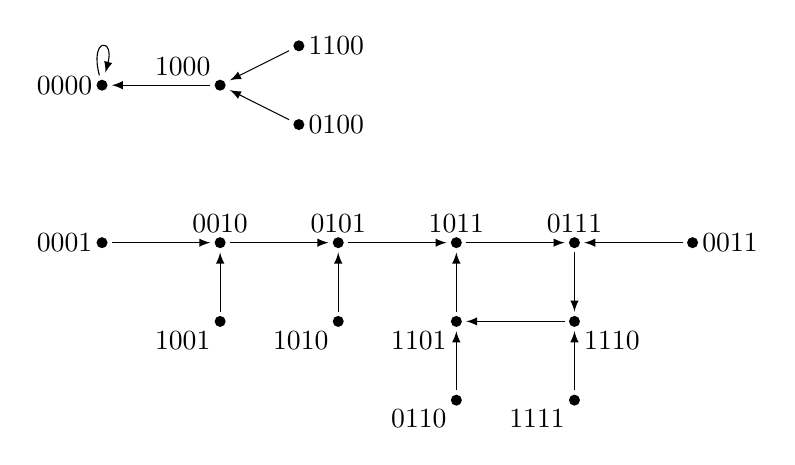
\begin{tikzpicture}[>=latex]
{\centering
\node (0000) at (0, 0)    {};
\node (0001) at (0, -2)   {};
\node (0010) at (1.5, -2) {};
\node (0011) at (7.5, -2)   {};
\node (0100) at (2.5, -0.5) {};
\node (0101) at (3, -2)   {};
\node (0110) at (4.5, -4)   {};
\node (0111) at (6, -2) {};
\node (1000) at (1.5, 0)    {};
\node (1001) at (1.5, -3) {};
\node (1010) at (3, -3)   {};
\node (1011) at (4.5, -2) {};
\node (1100) at (2.5, 0.5)   {};
\node (1101) at (4.5, -3) {};
\node (1110) at (6, -3) {};
\node (1111) at (6, -4) {};

\fill (0000)[right] circle (0.07) node[left]       {$0000$};
\fill (0001)[right] circle (0.07) node[left]       {$0001$};
\fill (0010)[left] circle (0.07) node[above]       {$0010$};
\fill (0011)[left] circle (0.07) node[right]       {$0011$};
\fill (0100)[left] circle (0.07) node[right]       {$0100$};
\fill (0101)[left] circle (0.07) node[above]       {$0101$};
\fill (0110)[left] circle (0.07) node[below left]  {$0110$};
\fill (0111)[left] circle (0.07) node[above]       {$0111$};
\fill (1000)[left] circle (0.07) node[above left]  {$1000$};
\fill (1001)[left] circle (0.07) node[below left]  {$1001$};
\fill (1010)[left] circle (0.07) node[below left]  {$1010$};
\fill (1011)[left] circle (0.07) node[above]       {$1011$};
\fill (1100)[left] circle (0.07) node[right]       {$1100$};
\fill (1101)[left] circle (0.07) node[below left]  {$1101$};
\fill (1110)[left] circle (0.07) node[below right] {$1110$};
\fill (1111)[left] circle (0.07) node[below left]  {$1111$};

\path[->] (0000) edge [loop above] node {} ();
\path[->] (0001) edge node {} (0010);
\path[->] (0010) edge node {} (0101);
\path[->] (0011) edge node {} (0111);
\path[->] (0100) edge node {} (1000);
\path[->] (0101) edge node {} (1011);
\path[->] (0110) edge node {} (1101);
\path[->] (0111) edge node {} (1110);

\path[->] (1000) edge node {} (0000);
\path[->] (1001) edge node {} (0010);
\path[->] (1010) edge node {} (0101);
\path[->] (1011) edge node {} (0111);
\path[->] (1100) edge node {} (1000);
\path[->] (1101) edge node {} (1011);
\path[->] (1110) edge node {} (1101);
\path[->] (1111) edge node {} (1110);

}
\end{tikzpicture}

\noindent Данный граф имеет структуру "циклы с подходами". Длины циклов: 1, 4. Это отображение не является взаимно однозначным.

\medskip

ЛРС $F_4 : (x_1, x_2, x_3, x_4) \rightarrow (x_2, x_3, x_4, x_1 \oplus x_3*x_4)$

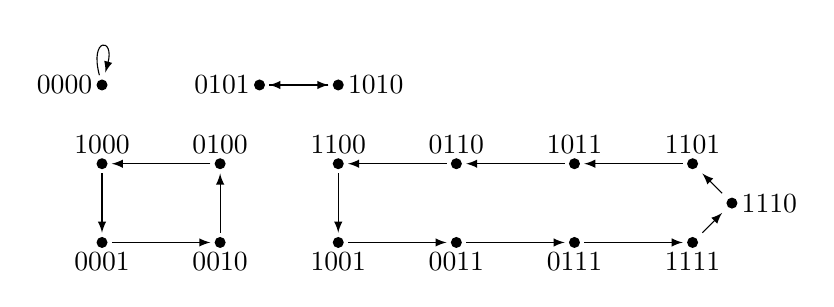
\begin{tikzpicture}[>=latex]
{\centering
\node (0000) at (0, 0)    {};
\node (0001) at (0, -2)   {};
\node (0010) at (1.5, -2) {};
\node (0011) at (4.5, -2)   {};
\node (0100) at (1.5, -1) {};
\node (0101) at (2, 0)   {};
\node (0110) at (4.5, -1)   {};
\node (0111) at (6, -2) {};
\node (1000) at (0, -1)    {};
\node (1001) at (3, -2) {};
\node (1010) at (3, 0)   {};
\node (1011) at (6, -1) {};
\node (1100) at (3, -1)   {};
\node (1101) at (7.5, -1) {};
\node (1110) at (8, -1.5) {};
\node (1111) at (7.5, -2) {};

\fill (0000)[right] circle (0.07) node[left]       {$0000$};
\fill (0001)[right] circle (0.07) node[below]       {$0001$};
\fill (0010)[left] circle (0.07) node[below]       {$0010$};
\fill (0011)[left] circle (0.07) node[below]       {$0011$};
\fill (0100)[left] circle (0.07) node[above]       {$0100$};
\fill (0101)[left] circle (0.07) node[left]       {$0101$};
\fill (0110)[left] circle (0.07) node[above]  {$0110$};
\fill (0111)[left] circle (0.07) node[below]       {$0111$};
\fill (1000)[left] circle (0.07) node[above]  {$1000$};
\fill (1001)[left] circle (0.07) node[below]  {$1001$};
\fill (1010)[left] circle (0.07) node[right]  {$1010$};
\fill (1011)[left] circle (0.07) node[above]       {$1011$};
\fill (1100)[left] circle (0.07) node[above]       {$1100$};
\fill (1101)[left] circle (0.07) node[above]  {$1101$};
\fill (1110)[left] circle (0.07) node[right] {$1110$};
\fill (1111)[left] circle (0.07) node[below]  {$1111$};

\path[->] (0000) edge [loop above] node {} ();
\path[->] (0001) edge node {} (0010);
\path[->] (0010) edge node {} (0100);
\path[->] (0011) edge node {} (0111);
\path[->] (0100) edge node {} (1000);
\path[->] (0101) edge node {} (1010);
\path[->] (0110) edge node {} (1100);
\path[->] (0111) edge node {} (1111);

\path[->] (1000) edge node {} (0001);
\path[->] (1001) edge node {} (0011);
\path[->] (1010) edge node {} (0101);
\path[->] (1011) edge node {} (0110);
\path[->] (1100) edge node {} (1001);
\path[->] (1101) edge node {} (1011);
\path[->] (1110) edge node {} (1101);
\path[->] (1111) edge node {} (1110);

}
\end{tikzpicture}

\noindent Граф имеет полностью цикловую структуру. Длины циклов: 1, 2, 4 и 9. Это отображение является взаимно однозначным.

\medskip

ЛРС $F_5 : (x_1, x_2, x_3, x_4) \rightarrow (x_2, x_3, x_4, x_1*x_3 \oplus x_2*x_4)$

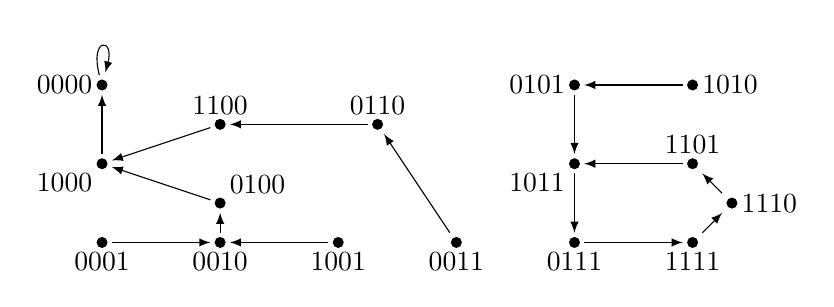
\begin{tikzpicture}[>=latex]
{\centering
\node (0000) at (0, 0)    {};
\node (0001) at (0, -2)   {};
\node (0010) at (1.5, -2) {};
\node (0011) at (4.5, -2)   {};
\node (0100) at (1.5, -1.5) {};
\node (0101) at (6, 0)   {};
\node (0110) at (3.5, -0.5)   {};
\node (0111) at (6, -2) {};
\node (1000) at (0, -1)    {};
\node (1001) at (3, -2) {};
\node (1010) at (7.5, 0)   {};
\node (1011) at (6, -1) {};
\node (1100) at (1.5, -0.5)   {};
\node (1101) at (7.5, -1) {};
\node (1110) at (8, -1.5) {};
\node (1111) at (7.5, -2) {};

\fill (0000)[right] circle (0.07) node[left]       {$0000$};
\fill (0001)[right] circle (0.07) node[below]       {$0001$};
\fill (0010)[left] circle (0.07) node[below]       {$0010$};
\fill (0011)[left] circle (0.07) node[below]       {$0011$};
\fill (0100)[left] circle (0.07) node[above right]       {$0100$};
\fill (0101)[left] circle (0.07) node[left]       {$0101$};
\fill (0110)[left] circle (0.07) node[above]  {$0110$};
\fill (0111)[left] circle (0.07) node[below]       {$0111$};
\fill (1000)[left] circle (0.07) node[below left]  {$1000$};
\fill (1001)[left] circle (0.07) node[below]  {$1001$};
\fill (1010)[left] circle (0.07) node[right]  {$1010$};
\fill (1011)[left] circle (0.07) node[below left]       {$1011$};
\fill (1100)[left] circle (0.07) node[above]       {$1100$};
\fill (1101)[left] circle (0.07) node[above]  {$1101$};
\fill (1110)[left] circle (0.07) node[right] {$1110$};
\fill (1111)[left] circle (0.07) node[below]  {$1111$};

\path[->] (0000) edge [loop above] node {} ();
\path[->] (0001) edge node {} (0010);
\path[->] (0010) edge node {} (0100);
\path[->] (0011) edge node {} (0110);
\path[->] (0100) edge node {} (1000);
\path[->] (0101) edge node {} (1011);
\path[->] (0110) edge node {} (1100);
\path[->] (0111) edge node {} (1111);

\path[->] (1000) edge node {} (0000);
\path[->] (1001) edge node {} (0010);
\path[->] (1010) edge node {} (0101);
\path[->] (1011) edge node {} (0111);
\path[->] (1100) edge node {} (1000);
\path[->] (1101) edge node {} (1011);
\path[->] (1110) edge node {} (1101);
\path[->] (1111) edge node {} (1110);

}
\end{tikzpicture}

\noindent Данный граф имеет структуру "циклы с подходами". Длины циклов: 1, 5. Это отображение не является взаимно однозначным.

\medskip